\chapter{自动加样系统控制方案的确定}
\section{总体控制系统的确定}
自动加样的实现离不开各功能模块之间的配合,配合好坏的程度取决于控制系统的设计。该控制系统由上位机、下位机控制器,功率驱动器,步进电机,位置检测器,液位传感器组成。其中,上位机、下位机控制器进行加样动作指令的接收与解析且二者信息双向流通,功率驱动器和步进电机作为被控对象,位置传感器和液位传感器作为回授元件,进行控制反馈的输入量。自动加样控制系统的结构关系图如\ref{fig:4-1}。

\begin{figure}[htbp!]
	\centering
	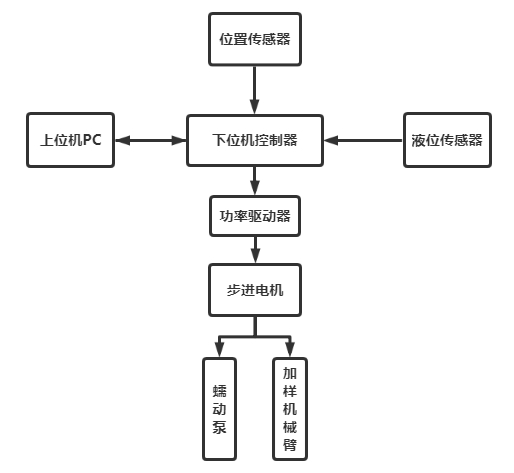
\includegraphics[height=9.5cm]{chap/figure/4-1.jpg}
	\caption{自动加样控制系统的结构关系简图}
	\label{fig:4-1}
\end{figure}

从自动加样控制系统的结构关系简图可知,本控制方案采取了半闭环控制系统,采用位置传感器和液位传感器将被控元件的位置情况反馈给控制器以保证加样精度和位置准确度。

\section{步进电机类型的选择}
步进电机是一种由数字信号驱动、以一定周期进行的同步电机,简单来说步进电机就是将输入的脉冲信号转动成转角或直线距离输出。其种类多种多样,按工作原理主要可以分为永磁式($PM$型)、磁阻式($VR$型),永磁感应式($HB$型)三大种类\supercite{bib12}。步进电机运动精度依赖于其最小步距角(分辨率)。对于永磁式步进电机,其转子由永磁体制作,多为两相结构,输出转矩小,其分辨率一般为45$^ \circ $、90$^ \circ $及11.25$^ \circ $等几种。对于磁阻式步进电机,其转子由加工成齿状的软铁构成,无惯性转矩响应快,其负荷惯性较小,其分辨率一般为15$^ \circ $。对于永磁感应式步进电机,转子由轴向磁化的磁铁制成且具有复极式磁极,兼具永磁式和磁阻式两种电机的优点,精确度高、转矩大、步进角度小。本文选用永磁感应式(混合型)步进电机。

永磁感应式步进电机一般有两相、三向和五相三种类型,相数越多分辨率越小,运动精度越高,价格也越来越贵。考虑成本和控制效果,本设计拟采用两相混合式步进电机,其分辨率为1.8$^ \circ $,另外对分辨率进行细分以补偿运动精度。经调研,我们选取$Leetro$公司的产品$DM5641E$,该步进电机产品体积小巧,适合用于医疗仪器、电控平移台、各种分析仪器、医疗泵、横流泵、蠕动泵、注射泵、机械手\supercite{bib14}等各种中小型自动化设备和仪器。$DM5641E$步进电机的产品参数如下表\ref{tab:4-1},实物图如\ref{fig:4-8},电机接线图如\ref{fig:4-9}。

\begin{table}[htbp]
	\centering
	\caption{$DM5641E$步进电机产品参数}
	\begin{tabular}{cc}
		\toprule
		\toprule
		内容    & 参数 \\
		\midrule
		相数  & 两相  \\
		步距角  & 1.8$^ \circ $ \\
		步距角精度  & $\pm5$ ${\rm{\% }}$ (整步,空载,无累积误差) \\
		径向最大负载  & 75$N$  \\
		轴最大负载  & 15$N$  \\
		\bottomrule
		\bottomrule
	\end{tabular}%
	\label{tab:4-1}%
\end{table}%

\begin{figure}[htbp] 
	\begin{minipage}[b]{0.5\textwidth} 
		\centering 
		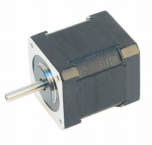
\includegraphics[width=0.6\textwidth]{chap/figure/4-8.jpg} 
		\caption{电机实物图} 
		\label{fig:4-8} 
	\end{minipage}% 
	\begin{minipage}[b]{0.5\textwidth} 
		\centering
		\centering 
		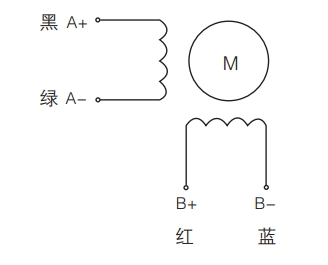
\includegraphics[width=0.8\textwidth]{chap/figure/4-9.jpg}  
		\caption{电机接线图} 
		\label{fig:4-9} 
	\end{minipage} 
\end{figure}



\section{步进电机的细分控制}
为保证加样的平稳进行,加样机械臂的加样动作一般速度较低,而二相混合式步进电机在速度较低的情况下由于分辨率(1.8$^ \circ $)相对较高,使用整步运行容易发生振动,造成样液在移送过程中出现滴漏而使检测结果出现误差,其振动效应甚至会导致机械部件的疲劳损坏\supercite{bib10}。根据步进电机的工作原理,增加步进电机的相数是一种可行的方法,但这又会导致成本上升;另一种可行的方案是对方波脉冲进行细分。

电机的细分技术最主要的目的是要减弱步进电机运动时的低频振动,但采用合理的细分方案能提高步进电机的精度,减轻低速运动时的振动。它的出现大大减轻了分辨率对步进电机相数的影响,提高了它的综合性能。细分技术的实质是将脉冲整波分割为若干个微波,以两相步进电机为例,它有$A$、$B$两个绕组。当绕组$A$通电时,其磁极(定子)产生磁场,吸引转子转动;绕组$B$通电时也是如此。输入脉冲作用一次,绕组的通电方向就变化一次,整步运行时其合成磁场方向如图\ref{fig:4-2},由图可知,每输入一个脉冲,电机转动90$^ \circ $。此时,$A$、$B$两相的通电顺序为\[A \to B \to \bar A \to \bar B \to A\]

\begin{figure}[htbp!]
	\centering
	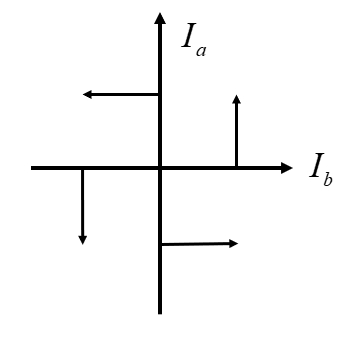
\includegraphics[height=8.5cm]{chap/figure/4-10.jpg}
	\caption{步进电机整步运行简图}
	\label{fig:4-2}
\end{figure}

细分控制即改变$A$、$B$相电流大小来改变合成磁场的夹角进而将一个整步分割多个微步,以四细分为例, $A$、$B$ 相绕组同时通电并改变它们的电流大小时,转子将停在$A$、$B$相磁极中间。其合成磁场方向如图\ref{fig:4-3}。由图可知,每输入一个脉冲,电机转动为 45$^ \circ $。此时,$A$、$B$两相的通电情况可以通过公式
$${I_a} = {I_i}\sin {\theta _i},{I_b} = {I_i}\cos {\theta _i} \eqno{(4-1)}$$

式中$I_a$,$I_a$为单相通电时电流大小,$I_i$为合成电流大小,${\theta _i}$为$A$、$B$ 相产生磁场的夹角。

研究表明\supercite{bib11},在同步带运动平台上,步进电机的四细分即能使其每步都能准确定位。本设计方案中细分控制采用八细分。

\begin{figure}[htbp!]
	\centering
	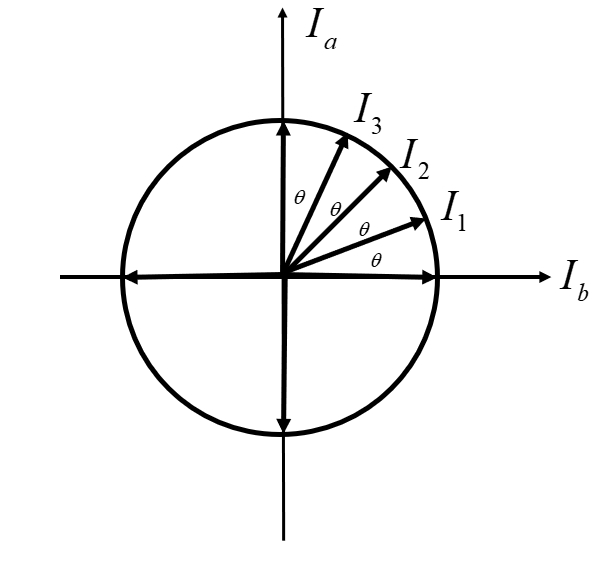
\includegraphics[height=8.5cm]{chap/figure/4-11.jpg}
	\caption{步进电机四分步运行简图}
	\label{fig:4-3}
\end{figure}

\section{步进电机的驱动控制分析}
步进电机分时通电,多相时序控制的工作原理决定了它不能在控制器输出的脉冲信号作用下直接工作。步进电机驱动器则针对了步进电机这一工作原理进行设计而产生的,它能通过截止和导通元件即环行分配器,将控制器输出的脉冲信号转换成能使步进电机各相绕组按一定顺序通电的脉冲信号。此外,环形分配器输出的脉冲功率很小不足以驱动电机(负载)工作,所以必须通过功率放大单元来获取大功率以驱动电机(负载)。驱动电路中的电流一般比较大,为了使其不影响控制电路,步进电机驱动器还有光电隔离电路以保证系统的正常工作。综上所述,步进电机的驱动器一般由光电隔离保护单元(接口电路),环形分配器,功率放大单元构成,其结构如图\ref{fig:4-6}

\begin{figure}[htbp!]
	\centering
	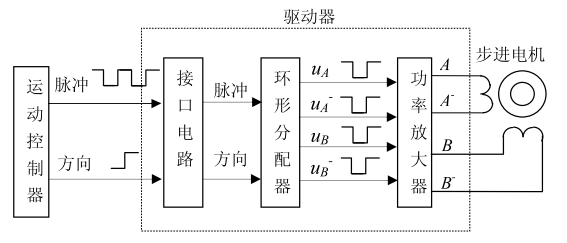
\includegraphics[height=6.5cm]{chap/figure/4-6.jpg}
	\caption{步进电机驱动器结构简图}
	\label{fig:4-6}
\end{figure}

\section{液位检测控制分析}
自动加样系统在取样和释样的过程中,加样针有一个检测位液深度的动作要求以保证试液精准、完整地取出和释放。目前,较为广泛使用的液面检测方法有两种,它们分别基于压力变化原理和电容变化原理。

基于压力变化式液位检测装置是根据传感器处于同种或异种的介质中的位置不同,其受到的压力也不同的原理设计的。如在本设计中,当液位传感器处于空气和试液的交界面时,压力值会发生跃变,并且随着传感器的深入压力值会越来越大,转换电路将压力值的变化转变为电流或电压的变化输出显示即完成检测任务。然而,由于检测的样液的种类多种多样,不同介质在同一位置引起的压力值也可能会不同,如此将会有非常大的误检发生概率。并且,基于压力值变化制作的传感器灵敏度低,需要另外设计变化量放大装置,不适用于微量加样系统。

基于电容变化式液位检测装置,利用两极板之间的介质的变化引起电容场值的变化来作为其工作原理。在本设计中,进入液面前后两极板之间的介质存在情况分别是只有空气和空气及样液混合介质,传感器进入不同的介质之后会引起电容值的变化。加样针即可制作为液面检测传感器\supercite{bib13},加样针的两筒璧作为电容场的两极板,其功能原理图如\ref{fig:4-7}。

\begin{figure}[htbp!]
	\centering
	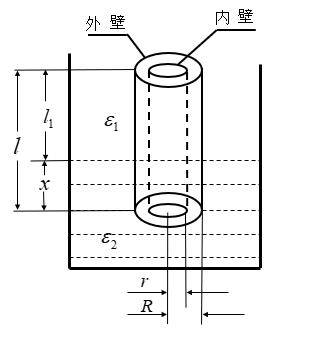
\includegraphics[height=8.5cm]{chap/figure/4-7.jpg}
	\caption{液面传感器功能简图}
	\label{fig:4-7}
\end{figure}

如图所示,当加样针部分进入试液的情况下,加样针总长度为$l$,外露在空气中部分长度为$l_1$,液面以下部分长度为$x$。假设空气的介电常数为${\varepsilon _1}$,试液的介电常数为${\varepsilon _2}$,总电容为$C$,空气部分电容为$C_1$,试液部分电容为$C_2$,则有:

$${C_1} = \frac{{2\pi {l_1}{\varepsilon _1}}}{{\ln \left( {\frac{R}{r}} \right)}},{C_2} = \frac{{2\pi x{\varepsilon _2}}}{{\ln \left( {\frac{R}{r}} \right)}} \eqno{(4-2)}$$

$$C = {C_1} + {C_2} \eqno{(4-3)}$$

整理式(5-2)和(5-3)可得

$$C = \frac{{2\pi \left( {l - x} \right){\varepsilon _1}}}{{\ln \left( {\frac{R}{r}} \right)}} + \frac{{2\pi x{\varepsilon _2}}}{{\ln \left( {\frac{R}{r}} \right)}} \eqno{(4-4)}$$

由式(5-4)可知,电容值$C$取决于加样针到达液面以下位置和两极板(加样针的内壁和外壁)之间介质的等效介电常数。事实上,当加样针由空气进入样液的瞬间,两极板之间的电容值会发生跃变,控制器捕获这一瞬间后,控制$Z$轴步进电机继续以一定速度驱动加样针下降至液面下某一位置(一般取$1-2mm$)停止即可,然后进行取样或释样动作。

